\documentclass[journal]{IEEEtran}
%\documentclass[11pt,twoside,a4paper]{article}

\usepackage{url}
\usepackage{amsmath}
\usepackage{amsfonts}
\usepackage{graphicx}
\usepackage[utf8]{inputenc}
\usepackage{subcaption}

%\usepackage[swedish]{babel}
\usepackage[backend=bibtex, citestyle=ieee, bibstyle=ieee]{biblatex}
\addbibresource{ref.bib}

% correct bad hyphenation here
\hyphenation{op-tical net-works semi-conduc-tor}

\begin{document}

\title{Homework 3 \\Semaphores}

\author{Hannes~Rabo, \textit{Information and Communication Technology}, KTH}


% The paper headers
\markboth{Homework 3 - Concurrent Programming (ID1217) - KTH}%
{}

% make the title area
\maketitle


% Note that keywords are not normally used for peerreview papers.
%\begin{IEEEkeywords}
% IEEE, IEEEtran, journal, \LaTeX, paper, template.
%\end{IEEEkeywords}

\IEEEPARstart{IN}{} this homework we create a concurrent application using semaphores that is fair and correct.

\newpage
\onecolumn

\begin{figure}[h]
\centering
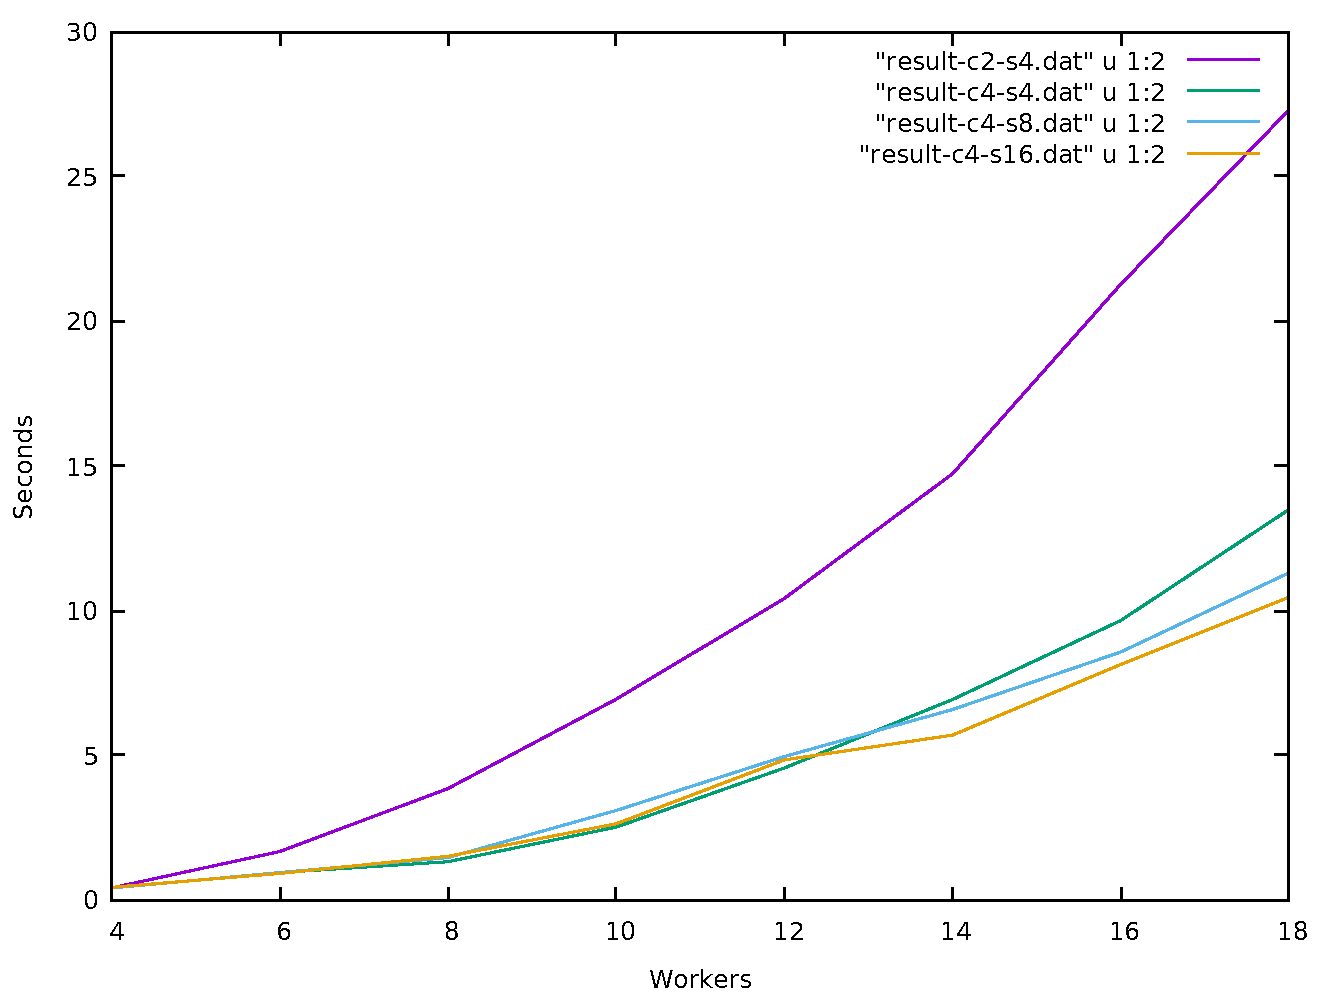
\includegraphics[width=\textwidth]{compare-total-time}
\caption{Total execution time as a function of number of workers (throughput)}
\label{fig:total}
\end{figure}


\begin{figure}[h]
	\centering
	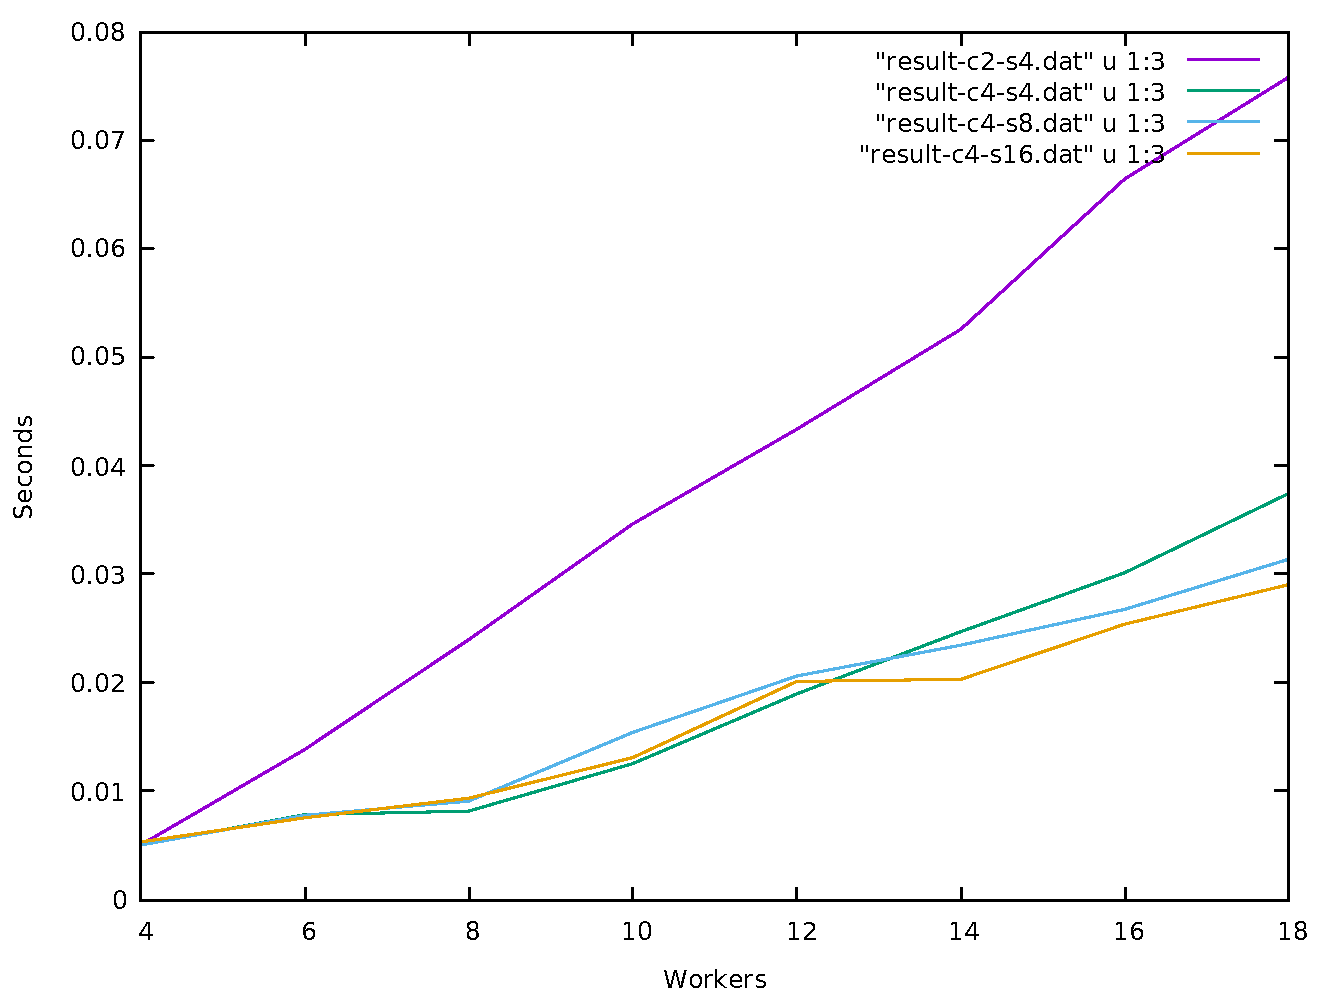
\includegraphics[width=\textwidth]{compare-avg}
	\caption{Average execution time as a function of number of workers (turnaround)}
	\label{fig:total}
\end{figure}

\printbibliography

%\appendices
%\section{Proof of the First Zonklar Equation}
%Appendix one text goes here.
%
%% you can choose not to have a title for an appendix
%% if you want by leaving the argument blank
%\section{}
%Appendix two text goes here.
%

\end{document}


